\documentclass{article}

\usepackage{amsthm}
\usepackage{graphicx}

\newtheorem{theorem}{Theorem}[section]
\newtheorem{proposition}[theorem]{Proposition}
\newtheorem{conjecture}[theorem]{Conjecture}

\theoremstyle{definition}
\newtheorem{example}[theorem]{Example}


\begin{document}
\section{Relations for the Reflection Quotient}
Represent the $(3,n)$-Torus knot as the closure of the braid word $(\sigma_1 \sigma_2)^n$. Consider the generating set $S = \{a,b,c\}$ where $a,b,c$ are as in Figure \ref{fig:generators}. 

\begin{figure}[ht]
\center{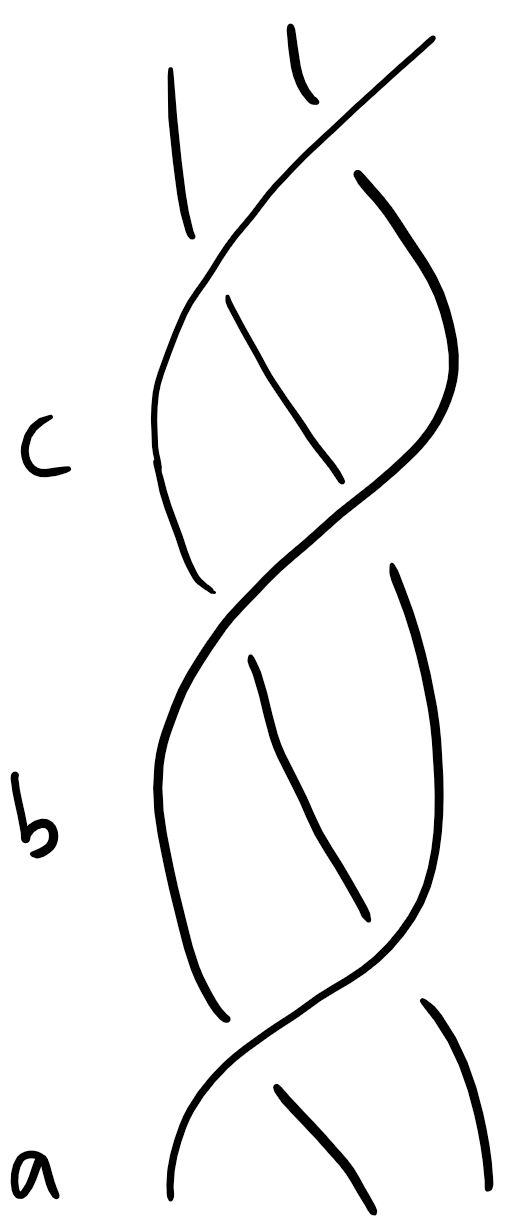
\includegraphics[scale = 0.3]
{figures/generators.png}}
\caption{\label{fig:generators} The generators of the reflection quotient}
\end{figure}

\begin{proposition}
The generating relations for a $(3,n)$-Torus link are
\begin{table}[ht]
\centering
\begin{tabular}{c|c|c}
{$T(3,3k)$} & {$T(3,3k+1)$} & {$T(3,3k+2)$} \\
\hline
& \\[-0.8em]
$(cba)^{k-1}cbabc(abc)^{k-1}a$ & $(cba)^{k-1}cbababc(abc)^{k-1}a$ & $(cba)^kc(abc)^ka$ \\
$(cba)^{k-1}cbc(abc)^{k-1}aba$ &  $(cba)^{k}bcb(abc)^{k}aba$ & $(cba)^kbab(abc)^kaba$\\
\end{tabular}
\end{table}
\end{proposition}

\begin{proof}
Use the twist relations from Figure \ref{fig:twistrelation}.
\begin{figure}[ht]
\center{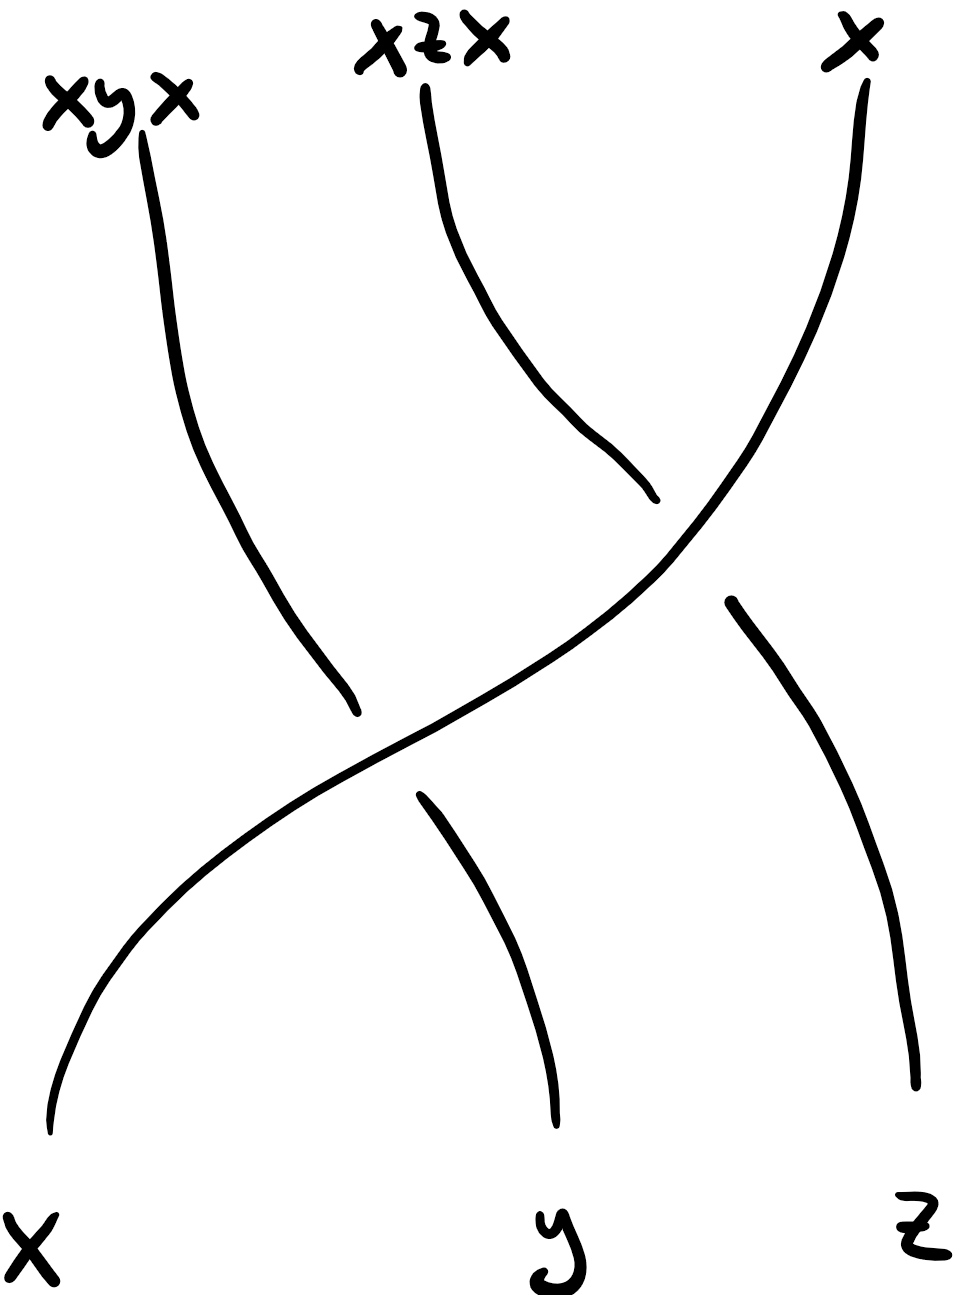
\includegraphics[scale = 0.22]
{figures/twistrelation.png}}
\caption{\label{fig:twistrelation} The relations induced by a twist}
\end{figure}
\end{proof}

\begin{example}
For the $(3,4)$-Torus knot, the above relations are $cbababca$ and $cbabcbabcaba$, so $|ab| = |bc| = 3$ and $|ac|=2$ yields a Coxeter quotient.
\end{example}

\begin{conjecture}
The $(n, n+1)$-Torus Knot has a Coxeter quotient isomorphic to $S_n$. More generally, so does the $(n, m(n+1))$-Torus Knot for all $m \geq 1$.
\end{conjecture}


\end{document}